\documentclass{acm_proc_article-sp}
%\usepackage{isolatin1}
\usepackage{amsmath}
\usepackage{amssymb}
\usepackage{epsfig,subfigure}
%\usepackage{acronym}
%\usepackage{graphics}
\usepackage{graphicx}
%\usepackage{times}
\usepackage{algorithm,algorithmic}
\usepackage{wrapfig}

\newcommand{\Ls}{L}
\newcommand{\Np}{N}
\newcommand{\p}{\gamma}
\newcommand{\groupr}[1]{\ensuremath{\left( #1 \right)}}
\newcommand{\groups}[1]{\ensuremath{\left[ #1 \right]}}
\newcommand{\groupc}[1]{\ensuremath{\left\{ #1 \right\}}}

\begin{document}

\title{Reducing the effect of sampling errors in UMDA\titlenote{(Produces the permission block, copyright information and page numbering). For use with ACM\_PROC\_ARTICLE-SP.CLS V2.6SP. Supported by ACM.}}
\numberofauthors{2}
%
% You can go ahead and credit authors number 4+ here;
% their names will appear in a section called
% "Additional Authors" just before the Appendices
% (if there are any) or Bibliography (if there
% aren't)

% Put no more than the first THREE authors in the \author command
\author{
%
% The command \alignauthor (no curly braces needed) should
% precede each author name, affiliation/snail-mail address and
% e-mail address. Additionally, tag each line of
% affiliation/address with \affaddr, and tag the
%% e-mail address with \email.
\alignauthor author 1\\
       \affaddr{Institute A}\\
       \affaddr{University B}\\
       \affaddr{Address}\\
       \email{Email@somewhere.domain}
%% \alignauthor author 2\\
%%        \affaddr{Institute A}\\
%%        \affaddr{University B}\\
%%        \affaddr{Address}\\
%%        \email{Email@somewhere.domain}
% \alignauthor J\"urgen Branke\\
%        \affaddr{Institute AIFB}\\
%        \affaddr{University of Karlsruhe}\\
%        \affaddr{Karlsruhe, Germany}\\
%        \email{branke@aifb.uni-karlsruhe.de}
% \alignauthor Clemens Lode\\
%        \affaddr{Institute AIFB (or whereever)}\\
%        \affaddr{University of Karlsruhe}\\
%        \affaddr{Karlsruhe, Germany}\\
%        \email{clemens@lode.de}
% \alignauthor Jonathan L. Shapiro\\
%        \affaddr{School of Computer Science}\\
%        \affaddr{University of Manchester}\\
%        \affaddr{Manchester, M13 9PL UK}\\
%        \email{Jonathan.Shapiro@manchester.ac.uk}
}

\maketitle

%------------------------------------------------------------------------------
% Abstract
%------------------------------------------------------------------------------
\begin{abstract}
  Estimation of distribution algorithms replace the typical crossover and
  mutation operators by constructing a probabilistic model and generating
  offspring according to this model. In previous studies, it has been shown
  that this generally leads to diversity loss due to sampling errors. In this
  paper, for the case of the simple Univariate Marginal Distribution Algorithm
  (UMDA), we propose and test several methods for counteracting diversity loss.
  The diversity loss can come in two phases: sampling from the probability
  model (offspring generation) and selection. We show that it is possible to
  completely remove the sampling error during offspring generation.
  Furthermore, we examine several plausible model construction variants which
  counteract diversity loss during selection and demonstrate that these update
  rules work better than the standard update on a variety of simple test
  problems.
\end{abstract}


%------------------------------------------------------------------------------
% Section 1: Introduction
%------------------------------------------------------------------------------

\section{Introduction}
\label{sec:intro}

Estimation of Distribution Algorithms (EDAs) are search algorithms
which use probability models instead of populations to search for
solutions of a problem. A population is generated by sampling from the
current probability model and selection is applied to this population.
The selected population is then used to generate the probability model for
the next generation, using methods developed by the statistical
machine learning community to build probability models from data.  A
range of EDAs have been proposed and developed, both for continuous
and discrete search spaces, and a number of successful applications
have been reported. For reviews, see the book~\cite{Larranaga2001} or
the review article~\cite{Pelikan:02}.

One known problem of EDAs is that they may suffer from ``premature
convergence''. As diversity is lost from the probability model, it
will not be restored. This was first shown
in~\cite{Gonzalez2002,Shapiro2003a} for PBIL, and has been shown to
hold generally for EDAs~\cite{Shapiro2006}.  The effect is analogous to genetic
drift\footnote{In population genetics, the term {\em drift} refers to
  the loss of genetic diversity due to finite population sampling} for
ordinary evolutionary algorithms, and it is most apparent when
operating on a flat fitness landscape, as the algorithm quickly
converges to a single solution.

The variance loss happens at two stages of the EDA: when the
population is generated by sampling from the probability
distribution, and when selection is applied to this population to generate the
probability model for the next generation.  In this paper,
we propose a number of ways to counteract this variance loss for the
example of the Univariate Marginal Distribution Algorithm (UMDA),
which is a typical yet simple EDA. However, we believe that similar
ideas can be applied also to more complex EDAs.

As we show, the variance loss in the offspring generation phase can be
easily removed by more intelligent sampling techniques. Counteracting
the variance loss due to selection is more difficult, and we propose
and empirically compare several approaches.

The paper is structured as follows. In Section~\ref{sec:umda} we give
a short introduction to UMDA and briefly recall the main results on
variance loss. Section~\ref{sec:generation} deals with removing
the variance loss from the offspring generation phase, while different
alternatives to reduce the variance loss in the model generation phase
are discussed in Section~\ref{sec:model}. The different proposed variants
are empirically compared in Section~\ref{sec:results}. The paper concludes
with a summary and some ideas for future work.

\section{UMDA}
\label{sec:umda}

The Univariate Marginal Distribution Algorithm (UMDA)
\cite{Muhlenbein1999} is an example of an estimation of distribution
algorithm (EDA) which acts on discrete variables and treats all
variables as independent. 

For simplicity, we consider binary strings of length $\Ls$. The
probability model treats each component of the string independently.
The parameters of the model are the probabilities that each component
takes the value $1$, denoted,
\begin{equation}
  \label{eq:UMDA_parameters}
  \p_i \equiv P(x_i = 1).
\end{equation}
At each iteration, $\Np$ strings will be sampled. The $i$th component of
the $\mu$th string is denoted $x_i^\mu$. Thus, the probability of
generating a string $\mathbf{x}^\mu$ can be written
\begin{equation}
  \label{eq:UMDAprob}
  P(\mathbf{x^\mu}) = \prod_{i=1}^{\Ls} \groups{\p_i {x_i^\mu}+
   \groupr{1-\p_i} {\groupr{1-x_i^\mu}}},
\end{equation}
and the probability of producing a population of $\Np$ strings is just
the product of Equation~(\ref{eq:UMDAprob}) over $\mu$.
                                                                                
Truncation selection is typically used 
although any selection operator can be utilized; the selected population consists of
a fraction $f$ of the best fitnesses in the population
(e.g. $f=0.5$). The parameters of the new model are given by the frequencies
of $1$'s at each site in the selected population.
\begin{equation}
  \label{eq:UMDA_learning}
\p_i \leftarrow \frac{1}{(f\Np)}{\sum_{\mu \in D_s} x_i^\mu },
\end{equation}
where $D_s$ is the data from the selected population. 
This choice of parameters maximizes the likelihood of the selected
data. 
Algorithm~\ref{alg:UMDA} shows the algorithm.
                                                                                
\begin{algorithm}
  \caption{Simple UMDA algorithm}
  \label{alg:UMDA}
   \begin{algorithmic}
    \STATE Set $\p_i\leftarrow 1/2$ for all $i=1 \ldots \Ls$;
    \REPEAT
      \STATE Sample $\Np$ strings according to Equation~(\ref{eq:UMDAprob}) to make a population $D$.
      \STATE Generate a new population $D_s$ from $D$ by selecting the
      $fN$ fittest strings.
      \FOR{$i=1$ to $\Ls$}
\STATE\begin{equation}
  \label{eq:pi}
\p_i \leftarrow \frac{1}{(f\Np)}{\sum_{\mathbf{x^\mu}\in D_s} x_i^\mu },
\end{equation}
\ENDFOR
\UNTIL{Stopping criterion met}
    \end{algorithmic}
\end{algorithm}

As has been shown in~\cite{Shapiro2005,Shapiro2006}, EDAs, and UMDA in
particular, suffer from a variance loss over generations. In brief,
instead of performing an unbiased search, they tend to search in
regions of the search space where they have searched before.  To see
why this is, consider what happens when the algorithm is run on a flat
landscape where all the states are equally good and selection has no
effect on the statistics of the population.  Obviously, the expected
mean of any property of the sampled population would be the mean of
the probability model. However, the variance of the sampled population
will be less than that of the probability model. It is very well known
that the variance of a sample of size $N$ has a expected value of size
$\sigma^2 (1-1/N)$ where $\sigma^2$ is the variance in the parent
distribution.  Most EDAs do not compensate for this; when the new
probability model is produced, it attempts to model the new population
and therefore has a reduced variance. When this is iterated
repeatedly, the variance of the sampled population gets smaller and
smaller and decays to zero. The probability model evolves to one which
can only generate identical configurations.

The diversity loss in UMDA occurs in two steps:
\begin{enumerate}
\item When sampling from the model distribution to generate the $N$
  offspring solutions. This happens independently of the optimization
  problem at hand and is due to the well-known fact that a sampled
  population has a variance smaller than that of the distribution from
  which it is sample. We refer to this as loss during offspring generation. 
\item When performing selection on the $N$ sampled solutions, i.e.\
  when choosing the better fraction of the population. It is clear
  that if selection is random, e.g.\ because there are several
  individuals with equivalent fitness, or because a randomized
  selection method is used, then this is just equivalent to
  sampling. In general, some diversity loss is due to the population
  focusing on fitter solutions, and some is random, but it is
  difficult to analyze and is problem dependent. We will use model generation
  rules to mitigate against this loss. 
\end{enumerate}

%Note that in UMDA, interdependencies between variables are not modeled, and thus
%for the remainder of the paper, it is mostly sufficient to consider a single
%bit position (as all other bit positions are handled analogously).

For the dynamics on a flat landscape, it was shown in \cite{Shapiro2006}
that if the diversity at a single bit position in a population of size
$\Np$ is $\sigma^2$ (as measured by the variance), then after removing
a fraction $(1-f)$ of the population by truncation selection, constructing a model
and generating a new population of size $\Np$, the variance is reduced
to $\sigma^2 \groupr{1-\frac{1}{f\Np}}$. In other words, the total variance
loss within one iteration on a flat landscape corresponds to the
factor
\begin{eqnarray}
\mathcal{L}_t=\groupr{1-\frac{1}{f\Np}}.
\end{eqnarray}

This is distributed on the two sources of sampling error as follows:
Because we know that sampling a population of size $\Np$ from a distribution reduces
the variance by a factor $(1-\frac{1}{\Np})$, the variance loss of generating
$\Np$ offspring involves a variance loss of 
\begin{eqnarray}
\mathcal{L}_g=\groupr{1-\frac{1}{\Np}}
\end{eqnarray}
The selection step thus is responsible for the remaining variance loss,
\begin{eqnarray}
\mathcal{L}_s=\frac{f\Np-1}{f\Np-f}.
\end{eqnarray}

In standard EAs, the sampling error in the case of
generational reproduction is usually reduced by stochastic universal
sampling~\cite{Bak87}. This idea has also been transferred to
steady-state EAs in~\cite{BCD99}. Of course, standard EAs usually have
a mutation operator which explicitly changes the statistics of the
current population towards a more randomized one. Many EDAs lack this,
attempting to faithfully reproduce the statistics of the current
population in the constructed probability model.

The importance of diversity loss in EDAs was probably first
investigated by Gonzalez and
collaborators~\cite{Gonzalez2001,Gonzalez2002}. The authors showed
that in PBIL, a independent variable EDA related to UMDA, once the
probability at a particular site got sufficiently close to zero or
one, the probability that the diversity would be restored at that site
can be arbitrarily close to zero. This could be avoided if the rate of
updating the probability model was sufficiently slow, so that the
diversity loss is slower than the search rate. However, how
slow this rate must be is very problem-dependent, as was shown
in~\cite{Shapiro2003a}. 

Several methods have been used to reduce diversity loss. Although the
early authors did not explicitly mention diversity loss, early EDAs
use selection mechanisms which update the probability model very
slowly. For example, in an early study of an EDA called
MIMIC~\cite{Baluja1997}, statistics about the populations visited were
maintained in a matrix and this matrix was used to build the
probability model. The current population had a (roughly) 1\% effect
on this matrix. Steady state selection was also used. There was some
evidence that the rate of model updating was more important that the
form of the probability model~\cite{Johnson2001}.

For UMDA, the rate of diversity loss depends
on the population size, and is avoided using a sufficiently large
population size. The appropriate population size is again problem
dependent with an exponential (in the string length) dynamic
range~\cite{Shapiro2005}. A wide range of EDAs,
including those which learn structural relationships between
variables, behave like UMDA in this regard~\cite{Shapiro2006}. 

An explicit approach to control diversity loss in EDAs was introduced by
Mahnig and M\"uhlenbein~\cite{Mahnig2001}. They used Laplace's method of
updating the probability model; a method which is considered further in
section~\ref{sec:laplace} of this paper. This approach is equivalent to a
Bayesian method of updating. It was shown to have an analogous effects to
mutation, and was deemed ``Bayesian mutation''. Like mutation, it is an
operator which when repeatedly applied converges to the random population.

Another approach is to impose a detailed-balance condition on the probability
updates~\cite{Shapiro2003b,Shapiro2005}. This approach is parameter-free and
completely removes diversity loss on a flat landscape and for some problems it
is very effective. However, it makes it difficult to sample the optimum in
some problem. Cross-validation using a second population to test
for diversity loss due to random sampling was employed by structure modeling
in~\cite{Wu2006}, to some effect, but was not applied in UMDA.


%JBR: Perhaps re-write the following for UMDA.
%As a consequence this algorithm does not always find a
%good solution even for very easy problems like \emph{one-max}.  This
%was first investigated by \citet{Gonzalez2001}. They showed that if
%the initial probability parameters are sufficiently close to $1$ or
%$0$, the probability that the global optimum is \emph{never} found can
%be arbitrarily close to $1$. This was shown for $N=L=2$, but it is
%easy to generalise for arbitrary string lengths and population sizes.
%In another paper~\citep{Gonzalez2002}, the authors show that in the
%one-max problem PBIL does converge to the optimum if the learning rate, $\alpha$, is sufficiently small. Thus, in
%combination, these papers show that the optimum is only found with
%sufficiently slow learning of the probability model.

%The question of when PBIL fails to converge to the optimum and how
%small learning rate needs to be has been answered for specific problems
%by~\citet{Shapiro2003a}. It was shown that PBIL does not converge to
%the global optimum unless the learning rate $\alpha$ is smaller than a
%critical value, $\alpha_c(L)$, which is a function of the string
%length and the specific problem. The choice of algorithmic parameters which
%avoids this depends very strongly on the problem, and so cannot be
%predicted in advance.

\section{Removing the variance loss due to sampling}
\label{sec:generation}

The variance loss due to sampling can be easily removed by ensuring
that the generated population has exactly $\Np \p_i$ individuals with bit $i$ set
to $''1''$. This can be achieved by simply generating all bits for all the 
$\Np$ individuals, and then randomly permuting the bits amongst the individual
in each bit position.
Also, note that because $\p_i$ are calculated according to Equation~\ref{eq:pi},
$\Np \cdot \p_i$ is always integer, and the variance loss can be removed completely.
Later on, we will propose alternative model construction rules for $\p_i$ which do
no longer have this property. In this case, we suggest to randomly round up or down
proportional to the rounding error. That is, $\Np \cdot \p_i$ is rounded up to
$\lceil \Np \p_i \rceil$ with probability $\Np \p_i - \lfloor \Np \p_i \rfloor$ and
rounded down otherwise. 

We call the proposed sampling mechanism {\em permutation sampling}.
The goal and effect is similar to the goal and effect of stochastic
universal sampling~\cite{Bak87} used for parent selection in generational
evolutionary algorithms, namely to remove sampling errors due to small sample sizes
(i.e., a small population size) as much as possible.

\section{Reducing the variance loss due to selection}
\label{sec:model}

As discussed in Section~\ref{sec:umda}, the variance loss due to
selection on a flat landscape corresponds to
$\mathcal{L}_s=\frac{f\Np-1}{f\Np-f}$.  In this section, we propose a
couple of ways to remove the effect of this variance loss.  Note that
it is not possible to remove the variance loss by intelligent
sampling, as we have done for the offspring generation, because we can
only select whole individuals, and the gene positions are thus
strongly interdependent.

\subsection{Loss correction}
\label{sec:correction}

One idea to remove the effect of the expected variance loss is to
bias the model to generate a larger variance. Because we model binomial distributions,
the variance of the probability
model at gene position $i$ is just $\sigma^2_i=\p_i(1-\p_i)$. To counteract the variance
loss, we would thus replace $\p_i$ by a $\p'_i$ such that the expected variance loss is
counterbalanced
\begin{eqnarray}
\p'_i(1-\p'_i) = \frac{\p_i(1-\p_i)}{ \mathcal{L}_s} \label{eq:pi2}
\end{eqnarray}
As in a binomial distribution the highest variance is obtained for $\p_i=0.5$ and
decreases towards 0 and 1,
this basically corresponds to moving $\p_i$ closer to 0.5.
Equation~\ref{eq:pi2} easily leads to
\begin{eqnarray}
\p'_{i,1/2}=\frac{1\pm\sqrt{1-4(1-\p_i)\p_i)/\mathcal{L}_s}}{2}
\end{eqnarray}
For this to be a valid expression, we require $1-4(-\p_i^2+\p_i)/\mathcal{L}_s\geq0$. This
is fulfilled only for $\p_i\leq \frac{1}{2}\left(1-\sqrt{1-\frac{f\Np-1}{f\Np-f}}\right)$ and
$\p_i\geq \frac{1}{2}\left(1+\sqrt{1-\frac{f\Np-1}{f\Np-f}}\right)$, in which case
we can use the above equation to counterbalance the expected variance loss.
For $\p_i$ within these bounds, a $\p'_i=0.5$ would not be sufficient to counterbalance
the variance loss, in which case we simply set $\p'_i=0.5$.

Overall, the corrected probability is calculated according to 
\begin{eqnarray}
\p'_i=\left\{\begin{array}{r@{\quad:\quad}l}
  \frac{1-\sqrt{1-4(1-\p_i)\p_i)/\frac{f\Np-f}{f\Np-1}}}{2} & \p_i\leq \frac{1}{2}\left(1-\sqrt{1-\frac{f\Np-1}{f\Np-f}}\right)\\
  \frac{1+\sqrt{1-4(1-\p_i)\p_i)/\frac{f\Np-f}{f\Np-1}}}{2} & \p_i\geq \frac{1}{2}\left(1+\sqrt{1-\frac{\Np-1}{\Np-f}}\right)\\
 0.5 & \mbox{otherwise}
\end{array} \right.
\end{eqnarray}

Figure~\ref{fig:correction} demonstrates how $\p_i'$ differs from $\p_i$. 
The correction 
depends on the population size, $\Np$, and is smaller for larger population sizes.
The strongest effect is for $\p_i$ close to 0.5, when $\p'_i$ is always moved back
to 0.5. At the extremes, i.e.\  for $\p_i\rightarrow 0$ and $\p_i\rightarrow 1$, the 
correction vanishes. This basically leads to a stronger exploration in the early phase
of the optimization, while allowing to fully converge eventually. 
In the following, we will denote this method as loss correction, or LC for short.

\begin{figure}
\centerline{
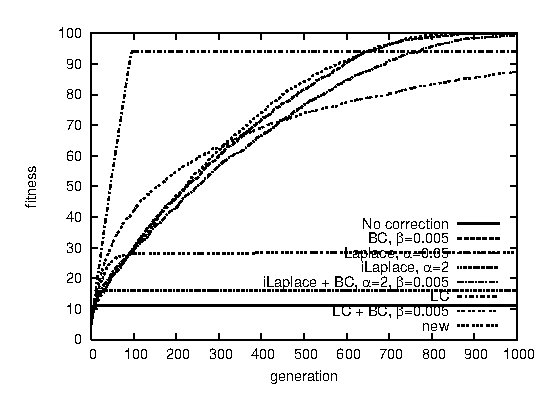
\includegraphics[width=0.4\textwidth]{graph_leading1169910391/graph_leading000_fitness.eps}}
\caption{Effect of loss correction (LC) on $\p_i$, assuming $\Np=10$.\label{fig:correction}}
\end{figure}

\subsection{Laplace correction}
\label{sec:laplace}

Bayesian statistics usually takes into account a prior distribution when
determining the probability model from observations made. In the absence of
any other knowledge, usually non-informative prior is used. For the binomial
distributions we consider, a commonly used prior is the beta distribution,
which is the conjugate prior for the binomial distribution (it is a special
case of the Dirichlet distribution). This would be integrated into the model
construction phase by replacing Equation~\ref{eq:pi} by
\begin{eqnarray}
\p_i=\frac{\sum_{\mathbf{x^\mu}\in D_s} x_i^\mu + \alpha}{f\Np + 2\alpha}\label{eq:laplace}
\end{eqnarray}
where $\alpha$ is a parameter which determines the strength of the
influence of the prior. In fact, the beta distribution is a
two-parameter distribution, but we only consider priors peaked at
$1/2$. 

The effect on $\p_i$ is depicted in Figure~\ref{fig:laplace} for
$\alpha=0.2$. As can be seen, the effect is quite different from the
loss correction described in the previous section. The probabilities are
almost not influenced near $\p_i=0.5$, but $\p_i$ is prevented from
converging completely to 0 or 1. This means that UMDA will never
completely converge but keep exploring, similar to an EA with a
minimum mutation probability. While this certainly improves the
exploratory power of the algorithm, it may dramatically delay the
algorithm finding the optimum, e.g.\ in OneMax, when the considered
string is long, and it becomes very unlikely to generate an offspring
consisting of all ones as long as $\p_i>\epsilon$.  Furthermore, we
know from the discussion above that the variance loss is at maximum
for $\p_i=0.5$, but the Laplace correction has basically no effect
there.
\begin{figure}
\centerline{
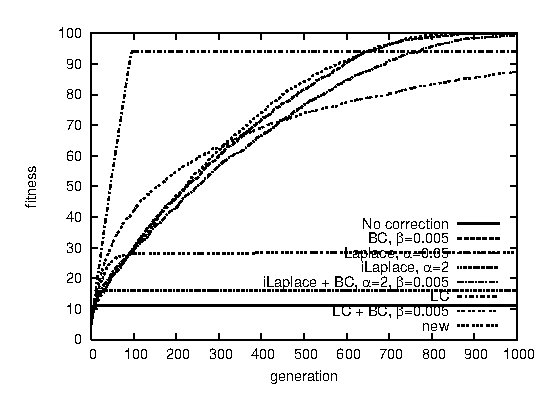
\includegraphics[width=0.4\textwidth]{graph_leading1169910391/graph_leading000_fitness.eps}}
\caption{Effect of Laplace correction on $p_i$, with $\Np=10$ and 
$\alpha=0.2$.\label{fig:laplace}}
\end{figure}



%JBR: Writing this, what do you think of the idea to add a mutation, i.e.\ increase 
%$\p_i$ by $\delta$ for $\p_i<0.5$ and decrease $\p_i$ by $\delta$ for $\p_i>0.5$?

\subsection{Incremental Laplace correction}
\label{sec:iLaplace}

The motivation for the Laplace correction was actually to take into
account a prior distribution. But except for the initial population,
the population has usually been generated from a Binomial distribution
with $\p_i\neq 0.5$. Thus, another idea would be to use beta
distribution peaked at $\p_i$ from the
last iteration as the prior distribution for the current generation, instead
of always assuming a prior distribution peaked at $1/2$.

More formally, we set
\begin{eqnarray}
\p_i(t)= \frac{\sum_{\mathbf{x^\mu}\in D_s} x_i^\mu + 2\alpha\p_i(t-1)}{f\Np + 2\alpha}\label{eq:ilaplace}
\end{eqnarray}

This can not be visualized in 2D, as it
additionally depends on the previous iteration's $\p_i$, but Figure~\ref{fig:iLaplace}
shows the plot for $\p_i(t-1)=0.25$. Basically, the incremental Laplace method,
or iLaplace method for short, discourages large deviations
from the previous distribution in either direction, and thus slows down convergence but
does not prevent it completely as with the Laplace correction from the previous section.


% Short version
As the beta distribution is a two-parameter family of functions, the
constraint that the prior distribution is peaked at $\p_i(t-1)$ can be realized
by a line in the parameter space. Equation~\ref{eq:ilaplace} is just one way
of parameterizing this line. Although any parametrization is equivalent when
$\p_i(t-1)$ is known, $\p_i(t-1)$ is a fluctuating
quantity. Equation~\ref{eq:ilaplace} is the parametrization which is unchanged
on a flat fitness landscape when averaged over sampling fluctuations.  

% Longer version continues
Specifically, Laplace's method is equivalent to using the value of $\p_i$
which maximizes the posterior distribution. In the standard parametrization of
the beta distribution, the peak of the posterior distribution is at  
\begin{equation}
\p_i(t)= \frac{\sum_{\mathbf{x^\mu}\in D_s} x_i^\mu + a}{f\Np + a + b} ,\label{eq:laplaceGeneric}
\end{equation}
where $a$ and $b$ are parameters. 
Using Laplace's method, we want this peaked at $1/2$ when there is no data,
which implies $a=b=\alpha$. With incremental Laplace, the peak is at
$\p_i(t-1)$, which implies $a\groups{1-\p_i(t-1)} = b\p_i(t-1)$.  By taking
$a=2\alpha \p_i(t-1)$ and $a+b=2\alpha$,  we insure that the update equation
is linear in $\p_i(t-1)$, and therefore has the desired average on a flat
space.  

\begin{figure}
\centerline{
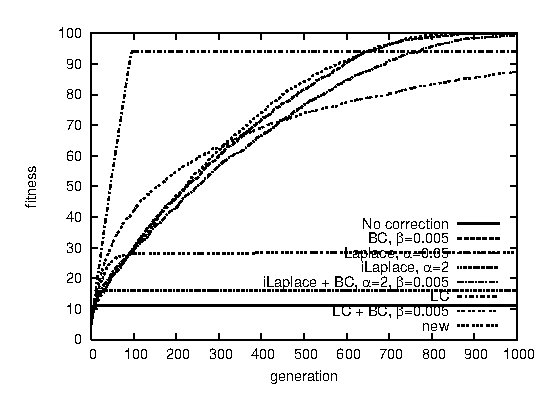
\includegraphics[width=0.4\textwidth]{graph_leading1169910391/graph_leading000_fitness.eps}}
\caption{Effect of incremental Laplace correction on $\p_i(t)$, at the example
of $\p_i(t-1)=0.25$.\label{fig:iLaplace}}
\end{figure}


\subsection{Boundary correction}
\label{sec:bc}

As has been explained above, the Laplace correction prevents UMDA from completely
converging, which has a great impact on algorithm performance (good and bad, depending
in the considered scenario). Because we wanted to separate the probability distribution
correction effect from the non-convergence effect, we introduce here the boundary
correction (BC), which does not influence the probability distribution except preventing
$\p_i$ from moving too close to either 0 or 1:
\begin{eqnarray}
\p'_i=\left\{\begin{array}{r@{\quad:\quad}l}
\beta & \p_i < \beta\\
1-\beta & \p_i > 1-\beta\\
\p_i & \mbox{otherwise}
\end{array}\right.
\end{eqnarray}.

For a visualization, see Figure~\ref{fig:bc}.
This method can be easily combined with the other correction methods, by simply
applying it as a second stage correction.

\begin{figure}
\centerline{
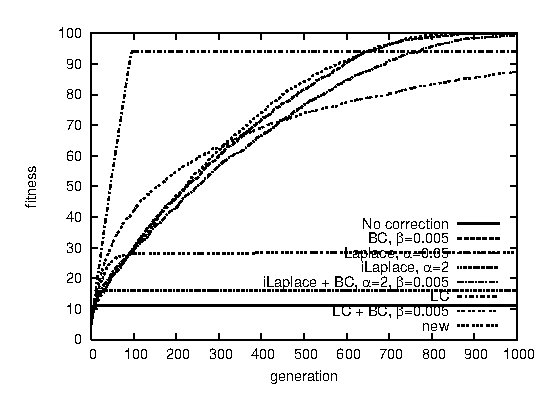
\includegraphics[width=0.4\textwidth]{graph_leading1169910391/graph_leading000_fitness.eps}}
\caption{Effect of boundary correction on $\p_i$, for $\beta=0.05$.\label{fig:bc}}
\end{figure}



\section{Empirical evaluation}
\label{sec:results}

We start our empirical evaluation in the first subsection with an examination of 
the effect of removing the sampling error
from the offspring generation phase. Then, in the remaining subsections, we will compare
the different model update strategies on a number of simple test problems,
namely 
\begin{itemize}
\item Flat landscape: all bit strings have equal fitness values, and consequently
selection is random.
\item OneMax: the fitness is the number of ones in the bit string.
\item LeadingOnes: the fitness is the number of leading ones in the bit string. Compared to
OneMax, this leads to a random drift of the later bit positions in the early generations, because
bit positions after the first zero have no influence on the fitness.
\item NK landscapes allow to set the level
of epistasis between bit positions. The fitness value is a sum of local fitness values $f_i$,
where $f_i$ is a randomly generated function based on bit position $i$ and the $k-1$ closest neighbors. 
In the tests below, we use $L=50$ and $k=5$.
\end{itemize}

As default values and unless specified otherwise, we use a population size of $\Np=20$, and problem size of $L=100, L=300$, and $L=500$ for the flat landscape, OneMax, and LeadingOnes, respectively.
Diversity is measured as
average variance over all bit positions.
All results reported below are averaged over 50 independent runs. 

\subsection{Removing the sampling error from offspring generation}
\label{sec:exactDistribution}

The undesired diversity loss due to sampling errors is most
significant on the flat landscape, because selection is purely
random. Figure~\ref{fig:ed} visualizes the dramatic diversity loss at
the example of a population of size $\Np=20$ and a problem of size $L=100$. 
According to the dashed line representing the standard UMDA, the
algorithm has basically converged to a single solution after about 40
iterations. Removing the sampling error for the offspring generation
step as proposed in Section~\ref{sec:generation} (solid line) can
not prevent the complete loss of diversity, but at least delays
it until after about 40 iterations. Nevertheless, such a delayed diversity
loss can greatly improve performance on problems which provide a fitness
gradient. Figure~\ref{fig:edOne} shows the fitness of the best solution
found so far for the OneMax problem, this time with problem size $L=300$. 
Neither of the two algorithms consistently finds
the optimum, but while the standard UMDA converges on average to a fitness of
241, using permutation sampling for the offspring generation pushes this
up to about 272.2.

%JBR: Shall we give this a better name than ``intelligent sampling''? After all,
%I think it will become standard, as SUS in EAs. What about ``Permutation Sampling''?

\begin{figure}
\centerline{
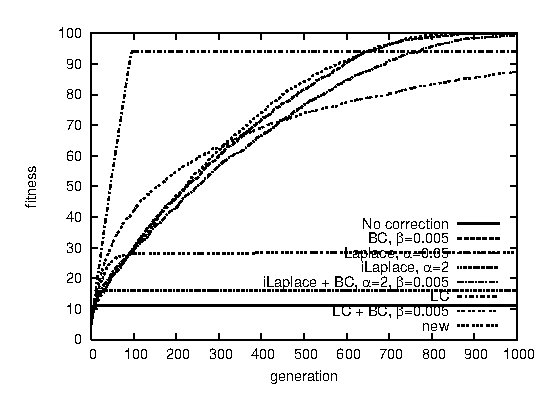
\includegraphics[width=0.4\textwidth]{graph_leading1169910391/graph_leading000_fitness.eps}}
%\includegraphics[width=0.4\textwidth]{graphs6/graph_flat1169862793/graph_flat000_diversity2.eps}}
\caption{Diversity loss on a flat landscape, $\Np=20, L=100$.\label{fig:ed}}
\end{figure}
\begin{figure}
\centerline{
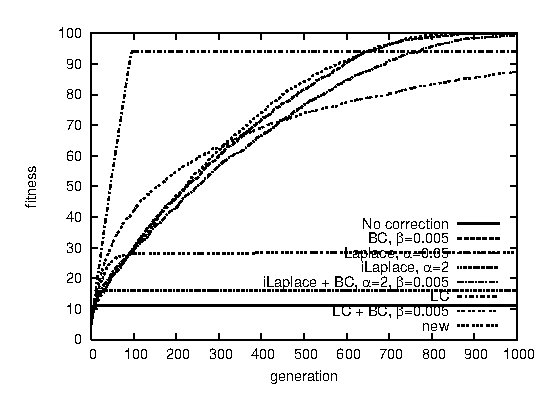
\includegraphics[width=0.4\textwidth]{graph_leading1169910391/graph_leading000_fitness.eps}}
\caption{Convergence curves for OneMax, best solution found so far, $\Np=20, L=300$.\label{fig:edOne}}
\end{figure}

Note that the removal of sampling error from the offspring generation phase
does not bias the algorithm in any way but simply helps it to do what
it is supposed to do. 
Because the variance loss depends on the population size $\Np$, the benefit from
permutation sampling will be larger the smaller the population size, but it should
always be beneficial.
We therefore recommend using this method under all circumstances,
and we use it as default in all subsequent tests to examine the different
model update strategies.

\subsection{Parameter settings for update strategies}
\label{sec:parameters}

Some of our proposed model update strategies have parameters, and in this section we
discuss how to set them appropriately.

The boundary correction (BC) basically corresponds to a minimal
mutation probability in evolutionary algorithms. And there, for simple
problems as the OneMax problem, a bit mutation rate of $1/L$ is
generally recommended (with $L$ denoting the string length of the
solution). For this reason, we will set $\beta=1/L$ in the experiments
reported below unless stated otherwise. The fact that this is a good parameter
setting was also confirmed in some additional empirical tests (not shown).

For Laplace correction, we assume that its main effect also lies in effectively
guaranteeing a minimal mutation probability. Therefore, we set $\alpha$ such that
the minimal mutation probability guaranteed equals $1/L$, i.e.\
\begin{eqnarray}
\frac{\alpha}{f\Np+2\alpha}=\frac{1}{L}
\end{eqnarray}
or
\begin{eqnarray}
\alpha=\frac{f\Np}{L-2}
\end{eqnarray}

Figure~\ref{fig:alpha} shows at the example of a OneMax problem
that BC and Laplace correction
with the recommended parameter setting indeed perform very similar,
and much better than the standard approach.
For larger parameter values, both approaches suffer, but Laplace
suffers significantly more than BC.

\begin{figure}
\centerline{
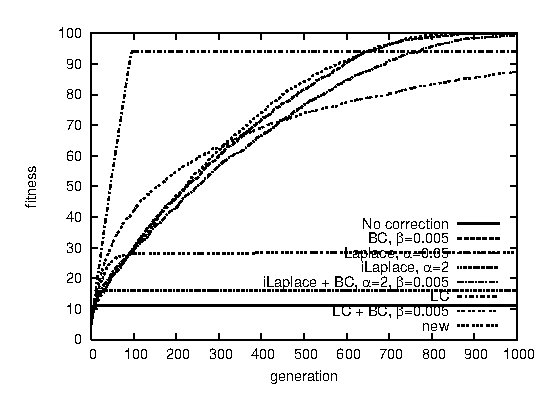
\includegraphics[width=0.4\textwidth]{graph_leading1169910391/graph_leading000_fitness.eps}}
\caption{Comparison of BC and Laplace correction on a OneMax problem, best solution found so far, $\Np=20, L=300$.\label{fig:alpha}}
\end{figure}

For iLaplace correction, we have no intuitive parameter setting, and indeed the optimal
parameter setting seems to depend very much on the problem at hand.
Figures~\ref{fig:ialpha} and \ref{fig:ialpha2} depict the convergence of the iLaplace
correction for different settings of $\alpha$ on the OneMax and LeadingOnes problems, respectively. While on the OneMax problem, we have a clear trade-off between convergence speed and
final solution quality (a larger $\alpha$ leads to slower convergence but better final solutions), on the LeadingOnes problem the slower convergence is almost not noticeable,
while there is a clear and dramatic increase in final solution quality.
If combined with BC, iLaplace yields only a marginal improvement over pure BC, but delaying convergence significantly.
Based on these observations,  we set $\alpha=2$ for
iLaplace in the following, unless specified otherwise.

\begin{figure}
\centerline{
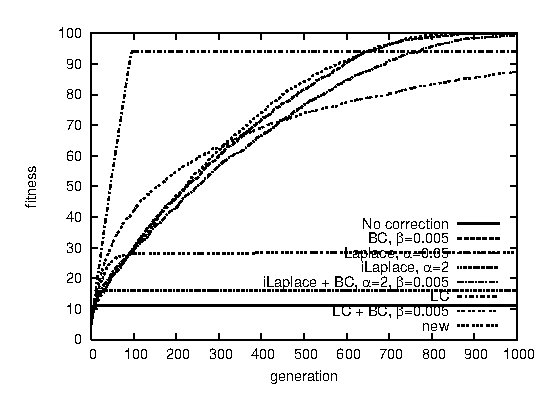
\includegraphics[width=0.4\textwidth]{graph_leading1169910391/graph_leading000_fitness.eps}}
\caption{The effect of parameter $\alpha$ on the iterative Laplace correction on 
a OneMax problem, $\Np=20, L=300$.\label{fig:ialpha}}
\end{figure}

\begin{wrapfigure}[r]
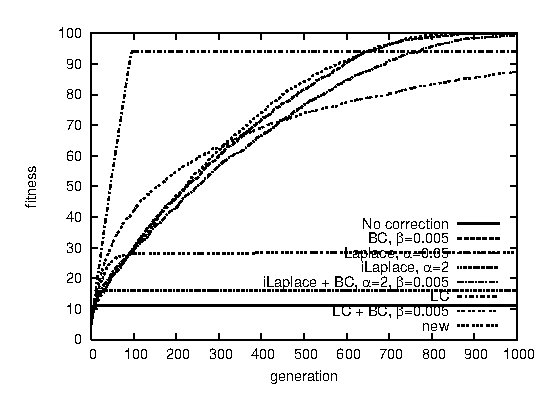
\includegraphics[width=0.4\textwidth]{graph_leading1169910391/graph_leading000_fitness.eps}
\caption{The effect of parameter $\alpha$ on the iterative Laplace correction on 
a LeadingOnes problem, $\Np=20, L=100$.\label{fig:ialpha2}}
\end{wrapfigure}


\subsection{Flat landscape}
\label{sec:flat}

Figure~\ref{fig:flat} compares the evolution of diversity for the different model update
strategies on the flat landscape.
Naturally, the BC and Laplace correction methods prevent a complete diversity loss, 
and we observe a somewhat higher convergence level for Laplace than for BC. LC and iLaplace
both fully converge, although slower than with the standard model update strategy.

The fact that the run with LC converges shows that this method is not able to fully
compensate the variance loss in the selection step. One reason is that it can not increase
variance beyond $\p_i=0.5$, another one is that it can only compensate for the {\em expected} loss, but not recover if the loss happened to be larger due to random fluctuations.
\begin{wrapfigure}
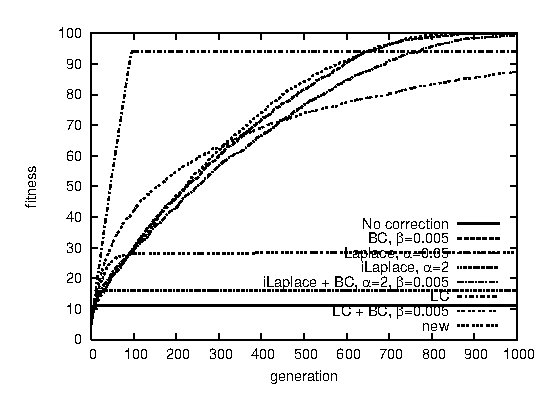
\includegraphics[width=0.4\textwidth]{graph_leading1169910391/graph_leading000_fitness.eps}
\caption{Comparison of the different model update strategies on the flat landscape, $\Np=20, L=100$.\label{fig:flat}}
\end{wrapfigure}

Interestingly, the diversity level is much higher than the minimum value of $\p_i=\beta$ would suggest. Considering $p(1-p)=0.1$ yields $p\approx 0.11$, i.e.\ a lot more bits are
mutated than we anticipated. This indicates that the results about optimal mutation rates do not readily carry over to BC settings in UMDA.
%Perhaps this means we have to think again about an appropriate
%level. Further idea: maintain a minimum diversity level in the population (instead of bit-wise).

\subsection{OneMax}
\label{sec:onemax}

On the OneMax problem, all proposed methods clearly outperform the standard model update
in terms of fitness obtained, see Figure~\ref{fig:oneFitness}. All methods which provide a minimal diversity threshold
get very close to the optimum. LC and LC+BC converge significantly slower than the other
methods. The diversity preservation by the pure LC and iLaplace strategies 
is not sufficient to prevent premature convergence, although they are still better than the standard method.
The fitness convergence is reflected also in the diversity convergence, see Figure~\ref{fig:oneDiversity}.

\begin{figure}[HT]
\centerline{
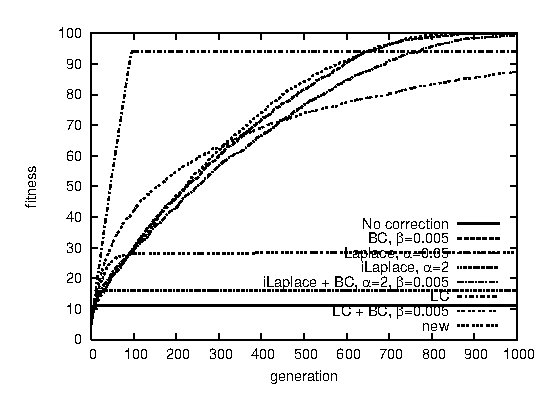
\includegraphics[width=0.4\textwidth]{graph_leading1169910391/graph_leading000_fitness.eps}}
\caption{Comparison of the different model update strategies on the OneMax landscape, best fitness found so far, $\Np=20, L=300$.\label{fig:oneFitness}}
\end{figure}
\begin{figure}[HT]
\centerline{
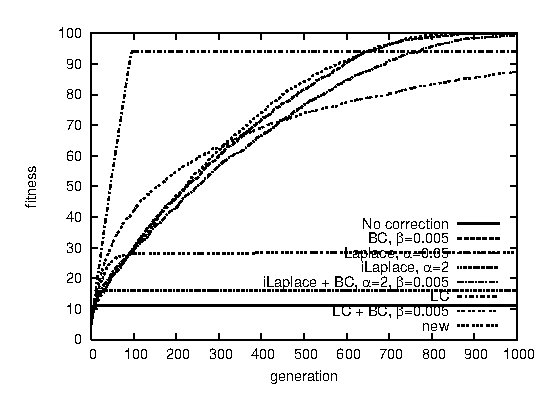
\includegraphics[width=0.4\textwidth]{graph_leading1169910391/graph_leading000_fitness.eps}}
\caption{Comparison of the different model update strategies on the OneMax landscape, $\Np=20, L=300$.\label{fig:oneDiversity}}
\end{figure}

\subsection{LeadingOnes}
\label{sec:leading}

The LeadingOnes problem has large plateaus consisting of all solutions
with the same number of leading ones. This puts it somewhere between the
flat landscape and OneMax, as it has a unique optimum, but at the same
time random selection plays an important role in the plateau
regions. Thus, it is important to maintain sufficient diversity in the
latter bits while the front bits are being optimized. On the other hand, too
much diversity is harmful at the end, as the the already found leading
ones are disturbed too much.

Figure~\ref{fig:leadingOnes} depicts the convergence of the different approaches. 
The standard update quickly converges to a fitness of only 10 (maximum is 100), 
which shows that LeadingOnes is a really difficult problem for EDAs.
The diversity preservation of pure LC and iLaplace improve fitness somewhat, but again can not
prevent premature convergence. The clear winners on this problem
are the approaches that maintain a minimum diversity level, i.e.\ 
Laplace and all methods combined with BC. They all reach a fitness level of about
80, differing in the time they require to find good solutions. Overall,
LC+BC seems to perform best.
Furthermore, we had set the default parameters based on OneMax. However, in LeadingOnes,
it is important to not disrupt the leading sequence of ones by too much exploration,
thus a smaller minimal mutation rate is appropriate for this problem.
When setting $\beta=0.005$ and $\alpha=0.05$, all the approaches maintaining
a minimum diversity are able to find the optimal solution with fitness 100
within 1000 iterations (not shown).

\begin{figure}
\centerline{
%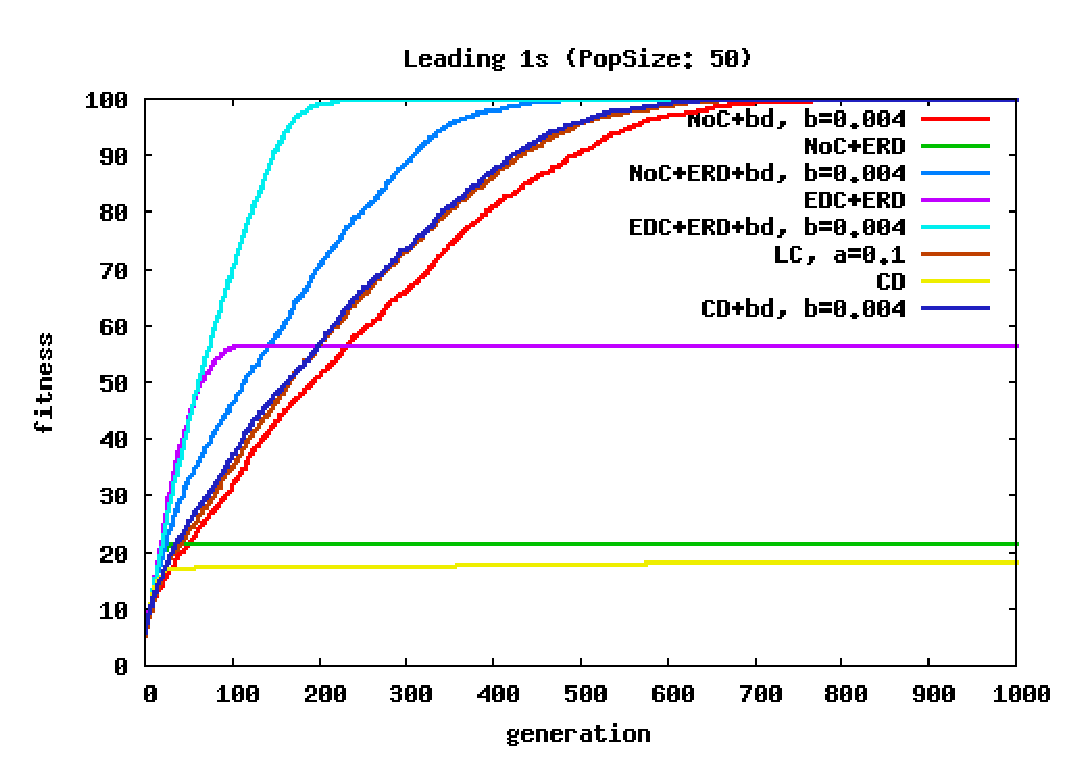
\includegraphics[width=0.4\textwidth]{graphs6/graph_leading1169868336/graph_leading000_fitness.eps}}
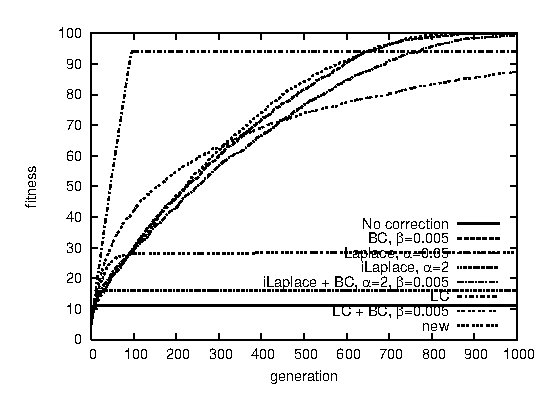
\includegraphics[width=0.4\textwidth]{graph_leading1169910391/graph_leading000_fitness.eps}}
\caption{Comparison of the different model update strategies on the LeadingOnes landscape, best fitness found so far, $\Np=20, L=100$.\label{fig:leadingOnes}}
\end{figure}


\subsection{NK landscapes}
\label{sec:nk}

On the NK landscape, the different model update strategies are
compared in Figure~\ref{fig:nk}.  As for the previous test problems, all update
strategies proposed in this paper outperform the standard approach
(solid line). Among the pure strategies, BC and Laplace perform very
well, followed by LC and then iLaplace. However, the latter two can be
combined with BC to ensure minimal mutation rates. While the
combination of iLaplace with BC is still worse than BC alone, the
combination of LC with BC yields the overall best results, although it
converges more slowly.
\begin{figure}
\centerline{
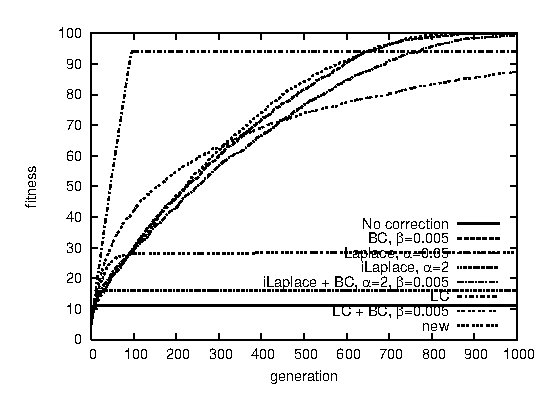
\includegraphics[width=0.4\textwidth]{graph_leading1169910391/graph_leading000_fitness.eps}}
%\includegraphics[width=0.4\textwidth]{Figures/nk.eps}}
\caption{Comparison of the different model update strategies on the NK landscape, best fitness found so far, $\Np=20, L=50, k=5$.\label{fig:nk}}
\end{figure}


\section{Conclusion}

Previous studies~\cite{Gonzalez2002,Shapiro2003a,Shapiro2006} have shown that the standard EDA
suffers from diversity loss due to sampling errors. In this paper, we have proposed a number
of methods to address this diversity loss. 

First, we have suggested an intelligent sampling technique, called permutation sampling, which is able to completely remove
the sampling error in the offspring generation phase of the algorithm. Since this method
otherwise leaves the algorithm unaltered, it should always be preferred to the standard
random offspring generation. 

The sampling error due to selection is more difficult to address. We have suggested a
number of intuitive ways to alter the model update, attempting to correct the
anticipated loss, taking into account a prior distribution, or ensuring a minimal
diversity level. The results in our empirical tests clearly show that all suggested
approaches seem to outperform the standard update on all problems, 
in most cases by a huge margin. 
The best model update strategy depends on the application, 
but the idea to correct for the expected diversity loss in combination with a minimal
ensured diversity level seems to preform best overall.

In the future, we plan to test our ideas more extensively also on real-world problems, and to extend the suggested methods to a larger alphabet, other selection mechanisms than truncation selection, and, more importantly, to more complex EDAs such as BOA.
Finally, it seems very promising to adapt the proposed methods also on dynamic
test problems, where diversity is particularly important.


\bibliographystyle{plain}
\bibliography{EDA}

\end{document}
